\documentclass[a4paper]{report}
% Shared preamble for the English probability and statistics documents.
% Based on the original course preamble. Compile with pdfLaTeX.
\usepackage[top=1.5cm,bottom=2cm,left=2cm,right=2cm]{geometry}
\usepackage[T1]{fontenc}
\usepackage{lmodern}
\usepackage[utf8]{inputenc}
\usepackage[english]{babel}

\usepackage{amsmath}
\usepackage{amssymb}
\usepackage{amsthm}
\usepackage{mathrsfs}
\usepackage{mathtools}
\usepackage{etoolbox}
\usepackage{tikz}
\usetikzlibrary{shapes.multipart,arrows.meta}
\usepackage{xcolor}
\usepackage{enumerate}
\usepackage[shortlabels]{enumitem}
\usepackage{hyperref}
\usepackage{version}
\usepackage{bbold}
\usepackage{fontawesome5}
\usepackage{fancyhdr}
\lfoot{}
\usepackage{natbib}
\usepackage{graphicx}
\usepackage{pdfpages}
\usepackage{authblk}
    
\usepackage{blindtext}
\usepackage{multicol}
\usepackage{collcell}
\usepackage{wrapfig}
\usepackage{blkarray}
\usepackage{cancel}
\usepackage{appendix}
\usepackage{float}
\makeatletter
\input{tex/assets/slashbox.sty}
\makeatother
\hypersetup{unicode,colorlinks,citecolor=red,filecolor=black,
  linkcolor=red,urlcolor=cyan}
\setlength{\columnsep}{1cm}
\pagenumbering{gobble}

\def\numtext#1{%
  \ifcase#1\or one\or two\or three\or four\or five\or six\or seven\or eight\or nine\or ten\or
  eleven\or twelve\or thirteen\or fourteen\or fifteen\or sixteen\or seventeen\or eighteen\or nineteen\or twenty\or Lots\fi}

\newcommand{\Byte}[1]{%
  \def\nodecontents{}%
  \foreach[count=\l] \k in {#1} {\xappto{\nodecontents}{\noexpand\nodepart{\numtext{\l}}\k}}%
  \node[rectangle split,rectangle split parts=8,rectangle split horizontal,draw] at (2,2){\nodecontents};}

\newcommand{\D}{{\mathrm{d}}}
\newcommand{\cE}{{\mathcal{E}}}
\newcommand{\cG}{{\mathcal{G}}}
\newcommand{\cX}{{\mathcal{X}}}
\newcommand{\cY}{{\mathcal{Y}}}
\newcommand{\cB}{{\mathcal{B}}}
\newcommand{\cF}{{\mathcal{F}}}
\newcommand{\cO}{{\mathcal{O}}}
\newcommand{\cS}{{\mathcal{S}}}
\newcommand{\cT}{{\mathcal{T}}}
\newcommand{\given}{\, \big| \,}
\newcommand{\cL}{{\mathscr{L}}}
\newcommand{\cD}{{\mathcal{D}}}
\newcommand{\cA}{{\mathscr{A}}}
\newcommand{\cP}{{\mathscr{P}}}
\newcommand{\cR}{{\mathscr{R}}}
\newcommand{\A}{{\mathcal A}}
\newcommand{\one}{\mathbb{1}}
\newcommand{\mathbbm}[1]{\mathbb{#1}}

\providecommand{\C}{}
\renewcommand{\C}{\mathbb C}
\newcommand{\R}{\mathbb R}
\newcommand{\Q}{\mathbb Q}
\newcommand{\N}{\mathbb N}
\newcommand{\T}{\mathbb T}
\newcommand{\F}{\mathbb F}
\renewcommand{\P}{\mathbb P}
\newcommand{\Z}{\mathbb Z}
\newcommand{\E}{\mathbb {E}}
\newcommand{\Pbb}[1]{\P\left( #1\right)}
\newcommand{\Ebb}[1]{\E\left[ #1\right]}

\newcommand{\lb}{\left (}
\newcommand{\rb}{\right )}
\newcommand{\lbb}{\left [}
\newcommand{\rbb}{\right ]}
\newcommand{\labs}{\left |}
\newcommand{\rabs}{\right |}
\newcommand{\lbrb}[1]{\lb #1 \rb}
\newcommand{\lbbrbb}[1]{\lbb#1\rbb}
\newcommand{\labsrabs}[1]{\labs#1\rabs}
\newcommand{\lbbrb}[1]{\lbb#1\rb}
\newcommand{\lbrbb}[1]{\lb#1\rbb}
\newcommand{\langlerangle}[1]{\langle#1\rangle}
\newcommand{\lbcurly}{\{}
\newcommand{\rbcurly}{\}}
\newcommand{\curly}[1]{\lbcurly#1\rbcurly}
\newcommand{\abs}{\labsrabs}
\newcommand{\ind}[1]{1_{#1}}
\newcommand{\indep}{\perp \!\!\! \perp}
\renewcommand{\d}{\, \mathrm{d}}

\newtheorem{theorem}{Theorem}
\newtheorem{problemCnt}{Lemma}
\theoremstyle{definition}
\newtheorem{problem}[problemCnt]{Problem}
\newtheorem{problembook}[problemCnt]{\faBook \,  Problem}
\newtheorem{problempencil}[problemCnt]{\faPencil* \,  Problem}
\newtheorem{problemstar}[problemCnt]{\faStar\,  Problem}
\newtheorem{problemstarpencil}[problemCnt]{\faStar \, \faPencil* \,   Problem}
\newtheorem{probleminteresting}[problemCnt]{\faSmile[regular] \,   Problem}
\newtheorem{solution}{Solution}

\newcommand{\fwcell}[1]{\makebox[\arraystretch\normalbaselineskip]{$#1$}}
\newenvironment{enumeratei}{\begin{enumerate}[(i)]}{\end{enumerate}}
\newenvironment{enumeratea}{\begin{enumerate}[(a)]}{\end{enumerate}}
\newenvironment{enumeraten}{\begin{enumerate}[\upshape 1.]}{\end{enumerate}}

% Compatibility helpers needed by a few files in the combined archive.
\AtBeginDocument{\noindent{\footnotesize English translation prepared with ChatGPT (OpenAI, GPT-6), 26 October 2026, for translation of the Bulgarian text into English and LaTeX formatting.
The Bulgarian originals remain the reference; translation may contain errors.}\par\smallskip}
\newcommand{\MissingGraphic}[1]{%
  \begin{center}\fbox{\parbox{0.82\linewidth}{\centering Missing source image: \texttt{#1}}}\end{center}}



\newif\ifshowsolutions
\showsolutionstrue
\begin{document}
\noindent Probability and Statistics, CS Year 3, 2020/2021 \hfill Test 2\ifshowsolutions: solutions\fi
\hrulefill
\begin{it}Your grade is 2 + the number of points. Time allowed: 3 hours. Good luck! Work on $(\Omega,\mathcal F,\P)$.\end{it}
\begin{problem}
A tank is filled with $X\in[0,1]$ units at the start of the week, and $Y$ units are consumed during the week. Their joint density is
\[f_{X,Y}(x,y)=3x\mathbbm1_{\{0\leq y\leq x\leq1\}}=\begin{cases}3x,&0\leq y\leq x\leq1,\\0,&\text{otherwise.}\end{cases}\]
\begin{enumerate}
\item (0.25 points) Find the probability that at most $1/2$ unit is added and more than $1/4$ consumed.
\ifshowsolutions
\par\textbf{Solution.}
\[\P(X<1/2,Y>1/4)=\int_{1/4}^{1/2}\int_{1/4}^x3x\,dy\,dx=\int_{1/4}^{1/2}3x(x-1/4)\,dx=\frac5{128}.\]
\fi
\item (0.75 points) Find $\mathrm{Cov}(X,Y)$.
\ifshowsolutions
\par\textbf{Solution.} For $x\in[0,1]$, $f_X(x)=\int_0^x3x\,dy=3x^2$, so $\E X=\int_0^1x3x^2\,dx=3/4$. Similarly, for $y\in[0,1]$,
\[f_Y(y)=\int_y^13x\,dx=\frac32(1-y^2),\qquad\E Y=\frac32\int_0^1y(1-y^2)\,dy=\frac38.\]
Finally,
\[\E[XY]=\int_0^1\int_0^xxy3x\,dy\,dx=\int_0^1\frac32x^4\,dx=\frac3{10},\]
so $\mathrm{Cov}(X,Y)=\E[XY]-\E X\E Y=3/160$.
\fi
\end{enumerate}
\end{problem}
\begin{problem} (1 point)
Information displays at public transport stops contain $10\times100$ diodes. Their high-quality components have exponentially distributed working lifetimes with mean 10 years. When fewer than 75\% work, the information is often unreadable and repair is required. What is the probability of repair being needed after three years?
\ifshowsolutions
\par\textbf{Solution.} Each lifetime is $\mathrm{Exp}(1/10)$, and its survival probability is
\[\P(\mathrm{Exp}(1/10)>3)=\int_3^\infty\frac1{10}e^{-x/10}\,dx=[-e^{-x/10}]_3^\infty=e^{-3/10}=:p.\]
The indicators $X_i=\mathbbm1_{\{\text{diode }i\text{ works after three years}\}}$ are $\mathrm{Ber}(p)$, with mean $p$ and variance $p(1-p)$. The finite variance and relatively large $n=1000$ allow the CLT approximation
\begin{align*}
\P\left(\sum_{i=1}^nX_i<750\right)&=\P\left(\frac{\sum X_i-np}{\sqrt{np(1-p)}}<\frac{750-np}{\sqrt{np(1-p)}}\right)\\
&\approx\P(N(0,1)<0.66)=\Phi(0.66)\approx74.54\%.
\end{align*}
\fi
\end{problem}
\begin{problem}
Model returns of assets $A,B,C$ as independent $N(3,2)$, $N(3,3)$ and $N(1,10)$ variables. You have five investment units.
\begin{enumerate}
\item (0.25 points) How should you allocate them to maximize expected profit?
\ifshowsolutions
\par\textbf{Solution.} Every $xA+(5-x)B$, $x\in[0,5]$, has the maximal expectation 15.
\fi
\item (0.25 points) Among those allocations, which minimizes variance?
\ifshowsolutions
\par\textbf{Solution.} $D(xA+(5-x)B)=2x^2+3(5-x)^2=5x^2-30x+75$, minimized at $x=30/10=3$.
\fi
\item (0.5 points) A risk-taking investor puts five units into independent asset $D\sim N(-2,20)$. What is the probability this outperforms part 2?
\ifshowsolutions
\par\textbf{Solution.} The portfolio in part 2 is $N(15,30)$, so
\[\P(N(15,30)<N(-10,500))=\P(N(25,530)<0)=\Phi(-25/\sqrt{530})\approx\Phi(-1.09)\approx13.79\%.\]
\fi
\end{enumerate}
\end{problem}
\begin{problem}
Travellers $X,Y$ go together from $A$ to $B$, then wait for buses to $C,D$, respectively. The travel times are $T_{AB}\sim\mathrm{Exp}(3)$, $T_{BC}\sim\mathrm{Exp}(4)$ and $T_{BD}\sim\mathrm{Exp}(5)$; the waiting times at $B$ are $T_C\sim\mathrm{Exp}(1)$ and $T_D\sim\mathrm{Exp}(2)$. All these times are independent. Let $\xi,\eta$ be the total journey times.
\begin{center}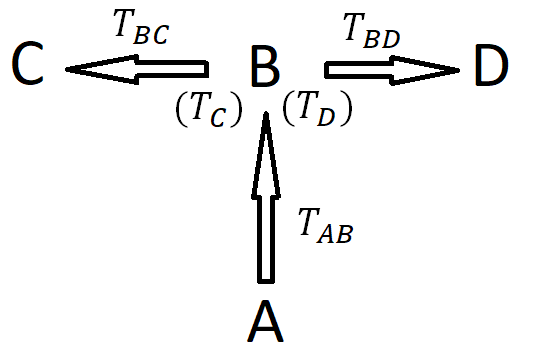
\includegraphics[width=7cm]{tex/assets/prob-stat/buses2.png}\end{center}
\begin{enumerate}
\item (0.25 points) Find $\P(T_C+\ln(\E T_D)>0)$.
\ifshowsolutions
\par\textbf{Solution.} As above, since $\ln(1/2)=-\ln2$, the probability is $\P(T_C>\ln2)=e^{-\ln2}=1/2$.
\fi
\item (0.75 points) Find $\mathrm{Cor}(\xi,\eta)$.
\ifshowsolutions
\par\textbf{Solution.} $\xi=T_{AB}+T_C+T_{BC}$ and $\eta=T_{AB}+T_D+T_{BD}$. Independence gives
\[D\xi=1/9+1+1/16=169/144,\qquad D\eta=1/9+1/4+1/25=361/900.\]
Direct calculation shows
\begin{align*}
\mathrm{Cov}(X_1+X_2,X_3)&=\E[(X_1+X_2)X_3]-\E[X_1+X_2]\E[X_3]\\
&=\mathrm{Cov}(X_1,X_3)+\mathrm{Cov}(X_2,X_3).
\end{align*}
Thus $\mathrm{Cov}(\xi,\eta)=\mathrm{Cov}(T_{AB},T_{AB})=DT_{AB}=1/9$, yielding
\[\mathrm{Cor}(\xi,\eta)=\frac{1/9}{\sqrt{D\xi D\eta}}=\frac{40}{247}\approx0.1619.\]
\fi
\end{enumerate}
\end{problem}
\end{document}
